
本章讨论紧\BookRecordIndex{T0358}辛流形中 $J$-全纯球面列的极限行为。最重要的结果是：每一列
$J$-全纯球面都有一个子列，依 Kontsevich\,\srcite{215} 的意义收敛到一个\BookRecordIndex{T0340}稳定映射。
第~\ref{sec:5-1} 节将详细讨论\BookRecordIndex{T0340}稳定映射的概念。在最初的工作~\srcite{160} 中，
\personlater{geluomofu}{格罗莫夫}{Gromov}使用了“\BookRecordIndex{T0181}尖点曲线”一词；它对应于\BookRecordIndex{T0340}稳定映射的
像，或者用代数几何的术语说，对应于一条\BookRecordIndex{T0216}可约曲线。第~\ref{sec:5-2} 节讨论\BookRecordIndex{T0141}格罗莫夫
收敛，特别地，我们将证明同伦类在这种极限下保持不变。随后在第~\ref{sec:5-3} 节证明：
每一列能量一致有界的 \BookRecordIndex{T0003}$J$-全纯曲线都有\BookRecordIndex{T0141}格罗莫夫收敛子列。

本章其余部分讨论\BookRecordIndex{T0340}稳定映射等价类的\BookRecordIndex{T0246}模空间
$\overline{\mathcal M}_{0,n}(M,A;J)$ 的结构，本书其他地方并不使用这些内容。我们的目标是
赋予这个空间一个由\BookRecordIndex{T0141}格罗莫夫收敛列产生的紧且\BookRecordIndex{T0212}可度量化的拓扑。第~\ref{sec:5-4} 节建立
格罗莫夫极限的唯一性，随后在第~\ref{sec:5-5} 节把收敛概念推广到\BookRecordIndex{T0340}稳定映射列
\sourcefootnote{原书把“建立格罗莫夫极限的唯一性”与“把收敛推广到\BookRecordIndex{T0340}稳定映射列”两项都归于
第 5.4 节；但第 5.4 节只证明唯一性，而\BookRecordIndex{T0340}稳定映射列的\BookRecordIndex{T0141}格罗莫夫收敛到第 5.5 节开头才定义，
故分别改作第 5.4 节与第 5.5 节。}。最后，第~\ref{sec:5-6} 节在
$\overline{\mathcal M}_{0,n}(M,A;J)$ 上引入\BookRecordIndex{T0142}格罗莫夫拓扑，并证明这个空间紧且\BookRecordIndex{T0212}可度量化。
为简单起见，本章始终假设黎曼曲面 $\Sigma$ 是球面。事实上，只要固定 $\Sigma$ 上的复结构
$j_\Sigma$，这些论证无须本质改变便适用于一般情形。在所有情形中，出现的\BookRecordIndex{T0275}气泡都是球面。

\section{\BookRecordIndex{T0340}稳定映射}\label{sec:5-1}
\zhindex{wendingyingshe}{稳定映射}

先回顾附录 D 中的一些定义。树是没有圈的连通图。我们把它看成一个有限集 $T$，配备关系
$E\subset T\times T$；两个顶点 $\alpha,\beta\in T$ 被 $E$ 联系（即
$\alpha E\beta$）当且仅当它们由一条边相连。$T$ 的一个 $n$-标号 $\Lambda$ 是函数
\[
  I\longrightarrow T,
  \qquad i\longmapsto\alpha_i,
\]
其中 $I:=\{1,\ldots,n\}$。这样的 $n$-标号也可描述为把指标集 $I$ 分拆成互不相交的子集
\[
  \Lambda_\alpha:=\{i\in I\mid\alpha_i=\alpha\}.
\]
有时允许更一般的指标集 $I$ 会很方便（见第~\ref{sec:5-5} 节）。对
$\alpha,\beta\in T$，区间 $[\alpha,\beta]\subset T$ 表示连接 $\alpha$ 与 $\beta$ 的
\BookRecordIndex{T0064}边链上的顶点集。当 $\alpha E\beta$ 时，删去连接 $\alpha$ 与 $\beta$ 的边后，以
$T_{\alpha\beta}$ 表示含有 $\beta$ 的\BookRecordIndex{T0417}子树，即
\[
  T_{\alpha\beta}:=\{\gamma\in T\mid\beta\in[\alpha,\gamma]\}.
\]
我们常把一棵 $n$-\BookRecordIndex{T0084}带标号树记作 $(T,\Lambda)$，或简记为 $T$。顶点数为 $\#T$，无向边数为
\[
  e(T):=\frac{\#E}{2}=\#T-1.
\]
\zhindex{daibiaoshu}{带标号树}
\zhindex{zishu}{子树}

\begin{definition}[\BookRecordIndex{T0340}稳定映射]\label{def:5-1-1}
设 $(M,\omega)$ 是紧\BookRecordIndex{T0358}辛流形，$J\in\mathcal J_\tau(M,\omega)$ 是被 $\omega$ \BookRecordIndex{T0372}驯服的
\BookRecordIndex{T0088}殆复结构，$n\ge0$ 是非负整数，并设 $(T,E,\Lambda)$ 是一棵 $n$-\BookRecordIndex{T0084}带标号树。
一个（以 $(T,E,\Lambda)$ 为模型的）$M$ 中带 $n$ 个\BookRecordIndex{T0066}标记点的亏格零稳定 $J$-全纯映射，
是一个元组
\[
  (\mathbf u,\mathbf z)
  =\bigl(\{u_\alpha\}_{\alpha\in T},
    \{z_{\alpha\beta}\}_{\alpha E\beta},
    \{\alpha_i,z_i\}_{1\le i\le n}\bigr),
\]
它由以下数据组成：一族由顶点 $\alpha\in T$ 标号的 $J$-全纯球面
$u_\alpha:S^2\to M$，一族由有向边 $\alpha E\beta$ 标号的\BookRecordIndex{T0191}节点
$z_{\alpha\beta}\in S^2$，以及 $n$ 个\BookRecordIndex{T0066}标记点 $z_1,\ldots,z_n\in S^2$；并且满足下列条件。

\emph{（\BookRecordIndex{T0191}节点）}若 $\alpha,\beta\in T$ 且 $\alpha E\beta$，则
\[
  u_\alpha(z_{\alpha\beta})=u_\beta(z_{\beta\alpha}).
\]
$\alpha$-球面上的\BookRecordIndex{T0191}节点集记作
\[
  Z_\alpha:=\{z_{\alpha\beta}\mid\alpha E\beta\}.
\]

\emph{（\BookRecordIndex{T0320}特殊点）}对每个 $\alpha\in T$，\BookRecordIndex{T0191}节点 $z_{\alpha\beta}$（$\alpha E\beta$）与
\BookRecordIndex{T0066}标记点 $z_i$（$i\in\Lambda_\alpha$）两两不同。它们称为\BookRecordIndex{T0320}特殊点。$\alpha$-球面上的\BookRecordIndex{T0320}特殊点集
记作
\[
  Y_\alpha:=Z_\alpha\cup\{z_i\mid\alpha_i=\alpha\}.
\]

\emph{（稳定性）}若 $u_\alpha$ 是常值函数，则 $\#Y_\alpha\ge3$。
\end{definition}

我们将看到，定义~\ref{def:5-1-1} 中的稳定性条件蕴含\BookRecordIndex{T0340}稳定映射的自同构群是有限群。不过要
注意，底\BookRecordIndex{T0072}层\BookRecordIndex{T0084}带标号树 $(T,E,\Lambda)$ 不必在附录 D 的意义下稳定，因为上面的稳定性条件只
涉及 $u_\alpha$ 为常值的分支（见附录 D.2 的式 (D.2.1)）。

每个映射 $u_\alpha$ 的定义域都是黎曼球面
$S^2\cong\mathbb C\cup\{\infty\}$。有时把这些定义域看成与二维球面微分同胚的、带复结构
的抽象二维流形 $\Sigma_\alpha$ 会有帮助；此时 $Y_\alpha$ 与 $Z_\alpha$ 是
$\Sigma_\alpha$ 的有限子集。考察高亏格\BookRecordIndex{T0340}稳定映射时，这一点很重要。不过，本章始终以标准
二维球面作为 $J$-全纯映射的定义域，并把 $\Sigma_\alpha$ 的元素写成
$(\alpha,z)\in T\times S^2$。因此，\BookRecordIndex{T0340}稳定映射 $(\mathbf u,\mathbf z)$ 的定义域可表示为商
\[
  \Sigma(\mathbf z):=T\times S^2/{\sim},
\]
其中 $T\times S^2$ 上的等价关系定义为：$(\alpha,z)\sim(\beta,w)$ 当且仅当
$\alpha=\beta$ 且 $z=w$，或者 $\alpha E\beta$、$z=z_{\alpha\beta}$ 且
$w=z_{\beta\alpha}$。以 $[\alpha,z]\in\Sigma(\mathbf z)$ 表示
$(\alpha,z)\in T\times S^2$ 的等价类。于是映射族 $\{u_\alpha\}_{\alpha\in T}$ 给出
映射
\[
  \Sigma(\mathbf z)\longrightarrow M,
  \qquad [\alpha,z]\longmapsto u_\alpha(z).
\]
子集 $[\{\alpha\}\times S^2]\subset\Sigma(\mathbf z)$ 称为 $\Sigma$ 的
$\alpha$-分支。若 $u_\alpha$ 为常值，则称它为\BookRecordIndex{T0384}幽灵气泡或\BookRecordIndex{T0382}幽灵分支。
\zhindex{youlingqipao}{幽灵气泡}
\zhindex{youlingfenzhi}{幽灵分支}

若 $(\mathbf u,\mathbf z)$ 是\BookRecordIndex{T0340}稳定映射，定义
\begin{equation}\label{eq:5-1-1}
  E(\mathbf u):=\sum_{\alpha\in T}E(u_\alpha),
  \qquad
  m_{\alpha\beta}(\mathbf u):=
  \sum_{\gamma\in T_{\alpha\beta}}E(u_\gamma),
  \qquad \alpha E\beta.
\end{equation}
见图~\ref{fig:5-1-1}。因此，$\mathbf u$ 的能量 $E(\mathbf u)$ 为零当且仅当所有映射
$u_\alpha$ 都是常值。在这种情形下，\BookRecordIndex{T0340}稳定映射 $(\mathbf u,\mathbf z)$ 可看成附录 D.3 的
定义 D.3.1 所指的\BookRecordIndex{T0339}稳定曲线与 $M$ 中一点所组成的二元组。对一般的 $\mathbf u$，定义域
$\Sigma(\mathbf z)$ 连同\BookRecordIndex{T0066}标记点 $[\alpha_i,z_i]$ 并不稳定。这时，\BookRecordIndex{T0191}节点曲线
$\Sigma(\mathbf z)$ 或元组
\[
  \mathbf z:=\bigl(\{z_{\alpha\beta}\}_{\alpha E\beta},
  \{\alpha_i,z_i\}_{1\le i\le n}\bigr)
\]
称为\BookRecordIndex{T0396}预稳定曲线。注意，加入新的\BookRecordIndex{T0066}标记点可以使\BookRecordIndex{T0396}预稳定曲线稳定化。
\zhindex{yuwendingquxian}{预稳定曲线}

\begin{figure}[htbp]
\centering
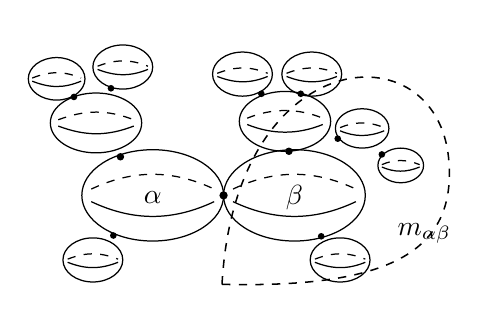
\begin{tikzpicture}[x=1cm,y=1cm,line width=0.45pt]
  \draw (-0.9,0) ellipse (0.9 and 0.58);
  \draw (0.9,0) ellipse (0.9 and 0.58);
  \draw[dashed] (-1.68,0.08) .. controls (-1.15,0.33) and (-0.65,0.33) .. (-0.12,0.08);
  \draw[dashed] (0.12,0.08) .. controls (0.65,0.33) and (1.15,0.33) .. (1.68,0.08);
  \draw (-1.68,-0.08) .. controls (-1.15,-0.33) and (-0.65,-0.33) .. (-0.12,-0.08);
  \draw (0.12,-0.08) .. controls (0.65,-0.33) and (1.15,-0.33) .. (1.68,-0.08);
  \node at (-0.9,-0.03) {$\alpha$};
  \node at (0.9,-0.03) {$\beta$};
  \fill (0,0) circle (1.5pt);

  \draw (-1.62,0.92) ellipse (0.58 and 0.38);
  \draw[dashed] (-2.1,0.96) .. controls (-1.75,1.09) and (-1.48,1.09) .. (-1.14,0.96);
  \draw (-2.1,0.88) .. controls (-1.75,0.75) and (-1.48,0.75) .. (-1.14,0.88);
  \fill (-1.31,0.49) circle (1.35pt);
  \draw (-2.12,1.48) ellipse (0.36 and 0.27);
  \draw[dashed] (-2.43,1.49) .. controls (-2.2,1.58) and (-2.03,1.58) .. (-1.81,1.49);
  \draw (-2.43,1.45) .. controls (-2.2,1.36) and (-2.03,1.36) .. (-1.81,1.45);
  \fill (-1.9,1.25) circle (1.2pt);
  \draw (-1.28,1.63) ellipse (0.38 and 0.28);
  \draw[dashed] (-1.6,1.64) .. controls (-1.37,1.73) and (-1.18,1.73) .. (-0.96,1.64);
  \draw (-1.6,1.60) .. controls (-1.37,1.51) and (-1.18,1.51) .. (-0.96,1.60);
  \fill (-1.43,1.36) circle (1.2pt);
  \draw (-1.66,-0.82) ellipse (0.38 and 0.28);
  \draw[dashed] (-1.98,-0.81) .. controls (-1.75,-0.72) and (-1.57,-0.72) .. (-1.34,-0.81);
  \draw (-1.98,-0.85) .. controls (-1.75,-0.94) and (-1.57,-0.94) .. (-1.34,-0.85);
  \fill (-1.4,-0.51) circle (1.2pt);

  \draw (0.78,0.94) ellipse (0.58 and 0.38);
  \draw[dashed] (0.3,0.98) .. controls (0.62,1.11) and (0.94,1.11) .. (1.26,0.98);
  \draw (0.3,0.90) .. controls (0.62,0.77) and (0.94,0.77) .. (1.26,0.90);
  \fill (0.83,0.56) circle (1.35pt);
  \draw (0.24,1.54) ellipse (0.38 and 0.28);
  \draw[dashed] (-0.08,1.55) .. controls (0.15,1.64) and (0.34,1.64) .. (0.56,1.55);
  \draw (-0.08,1.51) .. controls (0.15,1.42) and (0.34,1.42) .. (0.56,1.51);
  \fill (0.48,1.29) circle (1.2pt);
  \draw (1.12,1.54) ellipse (0.38 and 0.28);
  \draw[dashed] (0.8,1.55) .. controls (1.03,1.64) and (1.22,1.64) .. (1.44,1.55);
  \draw (0.8,1.51) .. controls (1.03,1.42) and (1.22,1.42) .. (1.44,1.51);
  \fill (0.98,1.29) circle (1.2pt);
  \draw (1.76,0.85) ellipse (0.34 and 0.25);
  \draw[dashed] (1.48,0.86) .. controls (1.67,0.94) and (1.84,0.94) .. (2.04,0.86);
  \draw (1.48,0.82) .. controls (1.67,0.74) and (1.84,0.74) .. (2.04,0.82);
  \fill (1.45,0.72) circle (1.2pt);
  \draw (2.25,0.38) ellipse (0.29 and 0.22);
  \draw[dashed] (2.01,0.39) .. controls (2.17,0.46) and (2.32,0.46) .. (2.49,0.39);
  \draw (2.01,0.36) .. controls (2.17,0.29) and (2.32,0.29) .. (2.49,0.36);
  \fill (2.01,0.52) circle (1.2pt);
  \draw (1.48,-0.82) ellipse (0.38 and 0.28);
  \draw[dashed] (1.16,-0.81) .. controls (1.39,-0.72) and (1.58,-0.72) .. (1.8,-0.81);
  \draw (1.16,-0.85) .. controls (1.39,-0.94) and (1.58,-0.94) .. (1.8,-0.85);
  \fill (1.24,-0.52) circle (1.2pt);

  \draw[dashed,line width=0.55pt]
    (-0.02,-1.13) .. controls (0.15,1.95) and (2.72,2.12) .. (2.86,0.45)
    .. controls (2.96,-0.72) and (2.1,-1.18) .. (-0.02,-1.13);
  \node at (2.55,-0.48) {$m_{\alpha\beta}$};
\end{tikzpicture}
\caption{\BookRecordIndex{T0340}稳定映射。}\label{fig:5-1-1}
\end{figure}

\begin{exercise}\label{ex:5-1-2}
\BookRecordIndex{T0178}加权树是配备\BookRecordIndex{T0291}权函数 $\mathrm w:T\to[0,\infty)$ 的\BookRecordIndex{T0084}带标号树 $(T,E,\Lambda)$。\BookRecordIndex{T0178}加权树的
总权是数
\[
  W(T):=\sum_{\alpha\in T}\mathrm w(\alpha).
\]
若每个满足 $\mathrm w(\alpha)=0$ 的顶点 $\alpha$ 都满足稳定性条件 (D.2.1)，则称\BookRecordIndex{T0178}加权树
$(T,E,\Lambda,\mathrm w)$ 稳定。利用引理 D.2.3 证明：对每棵至少有一条边的稳定加权
$n$-\BookRecordIndex{T0084}带标号树 $T$，边数满足
\[
  e(T)\le\frac{2W(T)}{\hbar}+n-3,
\]
其中 $\hbar$ 是其非零权的最小值。举例说明，当 $W(T)=0$ 时这个估计是尖锐的。特别地，
若 $\hbar$ 是命题~\ref{prop:4-1-4} 的常数，且 $(\mathbf u,\mathbf z)$ 是一个以 $T$ 为
模型、带 $n$ 个\BookRecordIndex{T0066}标记点的\BookRecordIndex{T0340}稳定映射，则
\begin{equation}\label{eq:5-1-2}
  e(T)\le\frac{2E(\mathbf u)}{\hbar}+n-3.
\end{equation}
\zhindex{jiaquanshu}{加权树}
\end{exercise}

\begin{exercise}\label{ex:5-1-3}
\begin{enumerate}[label=(\roman*),leftmargin=3em]
\item 证明：任意树 $T$ 的顶点 $\alpha_1,\ldots,\alpha_N$ 都可以适当排序，使得对每个
$i$，子集 $T_i:=\{\alpha_1,\ldots,\alpha_i\}$ 都是一棵树。证明任意顶点
$\alpha_1\in T$ 都可以选作这种排序的起点。
\item 给定 (i) 中的排序，证明对每个 $i\ge2$，都存在唯一指标 $j_i<i$，使
$\alpha_{j_i}E\alpha_i$。因此，一棵有 $N$ 个顶点的树可与整数向量
$\mathbf j=(j_2,\ldots,j_N)$ 等同，其中对每个 $i$ 都有 $1\le j_i<i$。
\item 令 $V_k:=\{i\mid j_i=k\}$，并注意对每个 $i\in V_k$ 都有 $k<i$。若 $k<i$，
证明 $\alpha_kE\alpha_i$ 当且仅当 $j_i=k$。
\end{enumerate}
\end{exercise}

\paragraph{\BookRecordIndex{T0413}重参数化群。}
\zhindex{chongcanshuhuaqun}{重参数化群}

\begin{definition}\label{def:5-1-4}
设\BookRecordIndex{T0340}稳定映射 $(\mathbf u,\mathbf z)$ 与 $(\widetilde{\mathbf u},\widetilde{\mathbf z})$ 分别以
\BookRecordIndex{T0084}带标号树 $(T,\Lambda)$ 与 $(\widetilde T,\widetilde\Lambda)$ 为模型。若存在\BookRecordIndex{T0304}树同构
$f:T\to\widetilde T$，以及函数
\[
  T\longrightarrow G=\operatorname{PSL}(2,\mathbb C),
  \qquad \alpha\longmapsto\phi_\alpha,
\]
即给每个顶点指定一个\BookRecordIndex{T0126}分式线性变换，使得
\begin{equation}\label{eq:5-1-3}
  \widetilde u_{f(\alpha)}\circ\phi_\alpha=u_\alpha,
  \qquad
  \widetilde z_{f(\alpha)f(\beta)}=\phi_\alpha(z_{\alpha\beta}),
  \qquad
  \widetilde z_i=\phi_{\alpha_i}(z_i),
\end{equation}
则称这两个\BookRecordIndex{T0340}稳定映射等价。由此可得，对每个 $\alpha\in T$，
$\Lambda_\alpha=\widetilde\Lambda_{f(\alpha)}$。
\end{definition}

对每棵\BookRecordIndex{T0084}带标号树 $T$，都有一个相应的群 $G_T$ 作用在以 $T$ 为模型的\BookRecordIndex{T0340}稳定映射集上，其轨道
空间就是相应的等价类集合。$G_T$ 的元素是元组
\[
  g=(f,\{\phi_\alpha\}_{\alpha\in T}),
\]
其中 $f$ 是满足
\[
  \Lambda_\alpha=\Lambda_{f(\alpha)}
\]
的 $T$ 的自同构，而对每个 $\alpha\in T$，$\phi_\alpha\in G$。所以在
$T=\widetilde T$ 的情形，$f$ 只能移动没有\BookRecordIndex{T0066}标记点的顶点 $\alpha$。群运算为
\[
  g'\cdot g
  =\left(f'\circ f,
    \{\phi'_{f(\alpha)}\circ\phi_\alpha\}_{\alpha\in T}\right).
\]
把 $f$ 看成给每个\BookRecordIndex{T0126}分式线性变换 $\phi_\alpha$ 指定靶球面的映射，并把
$\phi_\alpha$ 看成从二维球面 $\Sigma_\alpha$ 到 $\Sigma_{f(\alpha)}$ 的映射，会很有
帮助。群 $G_T$ 按
\[
  g\cdot(\mathbf u,\mathbf z)
  :=(\widetilde{\mathbf u},\widetilde{\mathbf z})
\]
作用在以 $T$ 为模型的\BookRecordIndex{T0340}稳定映射空间上，其中
$(\widetilde{\mathbf u},\widetilde{\mathbf z})$ 由式~\eqref{eq:5-1-3} 给出。显然，它的轨道
恰好定义以 $T$ 为模型的\BookRecordIndex{T0340}稳定映射的等价类。

定义~\ref{def:5-1-1} 中的稳定性条件保证每个\BookRecordIndex{T0340}稳定映射的\BookRecordIndex{T0342}稳定子群有限。通常这个\BookRecordIndex{T0342}稳定子群
是平凡的。不过，例如当 $T$ 有两个顶点 $\alpha,\beta$、没有标号且
$u_\alpha=u_\beta$ 时，它就是非平凡的。
\zhindex{wendingziqun}{稳定子群}

\begin{exercise}\label{ex:5-1-5}
群 $G_T$ 作用在以 $T$ 为模型的\BookRecordIndex{T0340}稳定映射的定义域 $\Sigma(\mathbf z)$ 所组成的集合上。
当 $T$ 是有五个顶点 $\alpha_1,\ldots,\alpha_5$、满足对 $i>1$ 有
$\alpha_1E\alpha_i$ 且没有标号的树时，描述这个作用的轨道。证明 $G_T$ 在这种定义域
$\Sigma(\mathbf z)$ 的集合上传递作用，当且仅当对每个 $\alpha$ 都有 $\#Z_\alpha\le3$。
\end{exercise}

\begin{exercise}\label{ex:5-1-6}
设 $T$ 是 $n$-\BookRecordIndex{T0084}带标号树，$(\mathbf u,\mathbf z)$ 是以 $T$ 为模型的\BookRecordIndex{T0340}稳定映射。证明
$G_T$ 的每个连通分支都有复维数 $3e(T)+3$。证明：当 $n+e(T)\le3$ 时，保持\BookRecordIndex{T0320}特殊点
（但不保持映射）的子群 $G_{T,\mathbf z}\subset G_T$ 的复维数为 $e(T)+3-n$；当
$n+e(T)\ge3$ 时，
\[
  e(T)+3-n\le\dim_{\mathbb C}G_{T,\mathbf z}\le2e(T).
\]
举例说明所有非负的可能值都会出现。
\end{exercise}

\paragraph{\BookRecordIndex{T0246}模空间。}
到 $M$ 的\BookRecordIndex{T0340}稳定映射构成范畴 $\mathcal{SC}_{0,n}(M;J)$ 的对象（字母
$\mathcal{SC}$ 可理解为“\BookRecordIndex{T0338}稳定范畴”）。从对象
$(\mathbf u,\mathbf z)\in\mathcal{SC}_{0,n}(M;J)$ 到
$(\widetilde{\mathbf u},\widetilde{\mathbf z})\in\mathcal{SC}_{0,n}(M;J)$ 的态射，是满足
定义~\ref{def:5-1-4} 中式~\eqref{eq:5-1-3} 的元组
$(f,\{\phi_\alpha\}_{\alpha\in T})$。因此，每个态射都是同构；两个\BookRecordIndex{T0340}稳定映射
$(\mathbf u,\mathbf z)$ 与 $(\widetilde{\mathbf u},\widetilde{\mathbf z})$ 等价，当且仅当
它们在范畴 $\mathcal{SC}_{0,n}(M;J)$ 中同构。定义~\ref{def:5-1-4} 的等价关系下，\BookRecordIndex{T0340}稳定映射
$(\mathbf u,\mathbf z)$ 的等价类记作 $[\mathbf u,\mathbf z]$。

现在固定球面同调类 $A\in H_2(M;\mathbb Z)$。若
$(\mathbf u,\mathbf z)\in\mathcal{SC}_{0,n}(M;J)$ 满足
\begin{equation}\label{eq:5-1-4}
  A=\sum_{\alpha\in T}u_{\alpha*}[S^2],
\end{equation}
则称它表示类 $A$。表示 $A$ 的\BookRecordIndex{T0340}稳定映射所组成的子范畴记作
\[
  \mathcal{SC}_{0,n}(M,A;J)
  :=\bigl\{(\mathbf u,\mathbf z)\in\mathcal{SC}_{0,n}(M;J)
  \bigm| \mathbf u\text{ 满足式~\eqref{eq:5-1-4}}\bigr\}.
\]
稍稍滥用逻辑学的标准约定，我们假装这些等价类构成一个集合，并把它记作
$\overline{\mathcal M}_{0,n}(M,A;J)$，或简记为
$\overline{\mathcal M}_{0,n}(A;J)$。（如附录 D.2 所述，若只考虑顶点取自某个给定集合的
树，这种说法就是完全严格的。）\BookRecordIndex{T0246}模空间 $\overline{\mathcal M}_{0,n}(M,A;J)$ 带有一个
称为\BookRecordIndex{T0142}格罗莫夫拓扑的自然拓扑。本章的目标是定义这一拓扑，并证明它使
$\overline{\mathcal M}_{0,n}(M,A;J)$ 成为紧且\BookRecordIndex{T0212}可度量化的空间。

\paragraph{\BookRecordIndex{T0072}层。}
对每棵\BookRecordIndex{T0084}带标号树 $T=(T,E,\Lambda)$ 与同调类 $A\in H_2(M;\mathbb Z)$，以
$\widetilde{\mathcal M}_{0,T}(M,A;J)$，或简记为
$\widetilde{\mathcal M}_{0,T}(A;J)$，表示所有以 $T$ 为模型且表示类 $A$ 的\BookRecordIndex{T0340}稳定映射所成的
空间。注意，$\widetilde{\mathcal M}_{0,T}(A;J)$ 是分别对应于 $A$ 的各种整同调类分解
\[
  A=\sum_{\alpha\in T}A_\alpha
\]
的子集之不交并。由命题~\ref{prop:4-1-5}，这些子集中只有有限多个非空。\BookRecordIndex{T0413}重参数化群 $G_T$
作用所得的商记作
\begin{equation}\label{eq:5-1-5}
  \mathcal M_{0,T}(M,A;J):=\mathcal M_{0,T}(A;J)
  :=\widetilde{\mathcal M}_{0,T}(A;J)/G_T.
\end{equation}
因此
\[
  \overline{\mathcal M}_{0,n}(A;J)
  =\bigcup_T\mathcal M_{0,T}(A;J),
\]
其中并取遍 $n$-\BookRecordIndex{T0084}带标号树的所有同构类。由练习~\ref{ex:5-1-2}，这个并中只有有限多个集合
非空。稍稍滥用术语，我们有时称 $\mathcal M_{0,T}(A;J)$ 为
$\overline{\mathcal M}_{0,n}(A;J)$ 的\BookRecordIndex{T0072}层；这并不表示
$\overline{\mathcal M}_{0,n}(A;J)$ 在严格意义下是分\BookRecordIndex{T0072}层空间。不过，第 6 章将证明：对一般的
与 $\omega$ \BookRecordIndex{T0348}相容的\BookRecordIndex{T0088}殆复结构 $J$，简单稳定元所成的子集
$\mathcal M^*_{0,T}(A;J)\subset\mathcal M_{0,T}(A;J)$ 是一个流形，相对于\BookRecordIndex{T0106}顶层的余维为
$2e(T)$。
\zhindex{ceng}{层}

与只有一个顶点的 $n$-\BookRecordIndex{T0084}带标号树 $T_n$ 对应的\BookRecordIndex{T0072}层称为\BookRecordIndex{T0106}顶层，记作
\[
  \mathcal M_{0,n}(A;J):=\mathcal M_{0,T_n}(A;J)
  =\widetilde{\mathcal M}_{0,n}(A;J)/G,
  \qquad
  \widetilde{\mathcal M}_{0,n}(A;J):=\widetilde{\mathcal M}_{0,T_n}(A;J).
\]
当 $A\ne0$ 且 $k=0,1$ 时，用第 3 章的术语，这些空间可描述为
\[
  \widetilde{\mathcal M}_{0,0}(A;J)=\mathcal M(A;J),
  \qquad
  \widetilde{\mathcal M}_{0,1}(A;J)=\mathcal M(A;J)\times S^2,
\]
以及
\[
  \mathcal M_{0,0}(A;J)=\mathcal M(A;J)/G,
  \qquad
  \mathcal M_{0,1}(A;J)=\mathcal M(A;J)\times_G S^2.
\]
当 $A=0$ 时，由于 $\widetilde{\mathcal M}_{0,k}(A;J)$ 中的元素还要满足稳定性条件，这些
恒等式不再成立。
\zhindex{dingceng}{顶层}

\personlater{geluomofu}{格罗莫夫}{Gromov}在 \srcite{160} 中引入了“\BookRecordIndex{T0181}尖点曲线”一词；它
对应于 $\overline{\mathcal M}_{0,0}(A;J)$ 中一个至少有两个分支的元素的像。\BookRecordIndex{T0181}尖点曲线可以
由定义域为任意\BookRecordIndex{T0191}节点黎曼曲面的映射来参数化。这个概念不如\BookRecordIndex{T0340}稳定映射精确，因为定义域的结构
丢失了。若目的仅仅是建立\BookRecordIndex{T0058}半正流形的\BookRecordIndex{T0143}格罗莫夫--威滕不变量的存在性，这一概念已经足够；但
不使用\BookRecordIndex{T0340}稳定映射，就无法看出这些不变量的完整结构（见第 7.5 节）。
\zhindex{jiandianquxian}{尖点曲线}

在代数几何中，人们用既约、不可约等词描述曲线。这里的重点仍是曲线的像，更确切地说，是
把曲线看成某些方程的解集。因此，每条曲线都是有限多个分支的并，每个分支还带有某个重数。
若曲线仅由一个重数为一的分支组成，就称它不可约；否则称它可约。若所有分支的重数都是一，
就称它既约。用我们的语言，一条曲线不可约，当且仅当它是某个单映射 $u:S^2\to M$ 的像。
\BookRecordIndex{T0176}既约曲线的概念也将很重要，因此我们引入\emph{\BookRecordIndex{T0184}简单稳定映射}
$(\mathbf u,\mathbf z)$：其中每个非常值分支 $u_\alpha$ 都是单映射，而且任意两个指标
$\alpha\ne\beta$ 的非常值映射之像 $\operatorname{im}u_\alpha$ 与
$\operatorname{im}u_\beta$ 都不重合。以 $T$ 为模型的\BookRecordIndex{T0184}简单稳定映射构成\BookRecordIndex{T0072}层
$\mathcal M_{0,T}(A;J)$ 的开子集 $\mathcal M^*_{0,T}(A;J)$，其性质将在第 6.2 节讨论。
显然，一条曲线在代数几何意义下既约，当且仅当它是一个\BookRecordIndex{T0184}简单稳定映射的像。最后要指出，
代数几何学家常用“\BookRecordIndex{T0386}有理曲线”表示亏格为零的曲线。

\begin{remark}[记号]\label{rem:5-1-7}
我们在一种语境中用字母 $\mathcal M$ 表示映射空间，在另一种语境中又用它表示映射等价类，
这多少有些不尽如人意。不过，两种用法都已约定俗成。许多论文（包括本书第一版）用类似
$\mathcal M(A;J)$ 的记号表示映射空间，而用 $\mathcal M_{0,n}(A;J)$ 与
$\overline{\mathcal M}_{0,n}(A;J)$ 表示\BookRecordIndex{T0340}稳定映射等价类的\BookRecordIndex{T0246}模空间也很常见。为了帮助读者
区分这两种记号，当 $\mathcal M(A;J)$ 表示映射空间时，我们绝不使用下标。此外，在需要
同时谈论这两类空间的场合，我们用 $\widetilde{\mathcal M}_{0,0}(A;J)$，而不用
$\mathcal M(A;J)$，表示 $J$-全纯球面空间。需要提醒读者，许多其他作者直接把
$\overline{\mathcal M}_{0,n}(A;J)$ 的元素 $[\mathbf u,\mathbf z]$ 称为\BookRecordIndex{T0340}稳定映射，而不再
明说这些元素是等价类。
\end{remark}

\paragraph{\BookRecordIndex{T0339}稳定曲线。}
若靶空间 $M$ 是一点，则
\[
  \overline{\mathcal M}_{0,n}
  :=\overline{\mathcal M}_{0,n}(\{\mathrm{pt}\},0;J)
\]
是带 $n$ 个\BookRecordIndex{T0066}标记点的亏格零\BookRecordIndex{T0339}稳定曲线的 Grothendieck--Knudsen \BookRecordIndex{T0246}模空间。附录 D 将详细讨论
这个\BookRecordIndex{T0246}模空间。它是复维数 $n-3$ 的光滑代数流形，并可写成各\BookRecordIndex{T0072}层的不交并
\[
  \overline{\mathcal M}_{0,n}=\coprod_T\mathcal M_{0,T},
\]
其中 $T$ 取遍稳定 $n$-\BookRecordIndex{T0084}带标号树的所有同构类。开\BookRecordIndex{T0072}层 $\mathcal M_{0,n}$ 由 $S^2$ 中 $n$ 个
互异\BookRecordIndex{T0066}标记点的所有构型对 $G=\operatorname{PSL}(2,\mathbb C)$ 的作用取商得到。每一\BookRecordIndex{T0072}层
$\mathcal M_{0,T}$ 的闭包 $\overline{\mathcal M}_{0,T}$ 都是
$\overline{\mathcal M}_{0,n}$ 中复余维为 $e(T)$ 的光滑子流形，而且任意两个这样的子流形
都\BookRecordIndex{T0136}干净相交（交集是子流形，交集的切空间等于二者切空间之交）。此外，子流形
$\overline{\mathcal M}_{0,T}$ 加性生成 $\overline{\mathcal M}_{0,n}$ 的上同调
\srcite{208}。\BookRecordIndex{T0246}模空间 $\overline{\mathcal M}_{0,3}$ 是一点，
$\overline{\mathcal M}_{0,4}$ 微分同胚于二维球面，而 $\overline{\mathcal M}_{0,5}$ 微分
同胚于 $S^2\times S^2$ 沿对角线上的三个点吹起所得的空间；见附录 D.7。

附录 D 说明了如何把 Grothendieck--Knudsen \BookRecordIndex{T0246}模空间 $\overline{\mathcal M}_{0,n}$ 嵌入若干
二维球面的乘积。在开\BookRecordIndex{T0072}层 $\mathcal M_{0,n}$ 上，这个嵌入由\BookRecordIndex{T0185}交比
\[
  w(z_i,z_j,z_k,z_\ell)
  =\frac{(z_j-z_k)(z_\ell-z_i)}{(z_i-z_j)(z_k-z_\ell)}
  \in\mathbb C\cup\{\infty\}
\]
给出。只要 $z_i,z_j,z_k,z_\ell$ 中没有三个相等，这个定义仍有意义，而且得到一个在 $G$
作用下不变的映射。例如，由于 $w(0,1,\infty,z)=z$，\BookRecordIndex{T0185}交比给出自然微分同胚
$\overline{\mathcal M}_{0,4}\to S^2$。附录 D.4 把\BookRecordIndex{T0185}交比延拓为函数
\[
  w_{ijk\ell}:\overline{\mathcal M}_{0,n}\longrightarrow S^2,
\]
具体如下。对每个顶点 $\alpha\in T$ 与每个指标 $i\in\{1,\ldots,n\}$，定义
$z_{\alpha i}\in S^2$ 为 $\alpha$-球面上指向\BookRecordIndex{T0066}标记点 $z_i$ 的元素，即
\begin{equation}\label{eq:5-1-6}
  z_{\alpha i}:=
  \begin{cases}
    z_i, & \alpha_i=\alpha,\\
    z_{\alpha\beta}, & \alpha_i\in T_{\alpha\beta}.
  \end{cases}
\end{equation}
对任意四个指标 $i,j,k,\ell$，都存在顶点 $\alpha$，使得
$z_{\alpha i},z_{\alpha j},z_{\alpha k},z_{\alpha\ell}$ 中没有三个相等；而且所得\BookRecordIndex{T0185}交比与这类
顶点 $\alpha$ 的选择无关。可以把得到的函数 $w_{ijk\ell}$ 看成遗忘除
$i,j,k,\ell$ 所标号者以外全部\BookRecordIndex{T0066}标记点的\BookRecordIndex{T0377}遗忘映射
$\overline{\mathcal M}_{0,n}\to S^2:=\overline{\mathcal M}_{0,4}$。这些函数给出上述嵌入，
也可以用来定义 $\overline{\mathcal M}_{0,n}$ 上的拓扑（见附录 D.5）。此外，每一\BookRecordIndex{T0072}层
$\mathcal M_{0,T}$ 的闭包 $\overline{\mathcal M}_{0,T}$ 映到一个复余维为 $e(T)$ 的复
子流形上，而 $\mathcal M_{0,n}$ 在 $\overline{\mathcal M}_{0,n}$ 中开且稠密。因此，
$\overline{\mathcal M}_{0,n}$ 的确是 $\mathcal M_{0,n}$ 的自然紧化。

\paragraph{\BookRecordIndex{T0377}遗忘映射。}
当 $n\ge3$ 时，有\BookRecordIndex{T0377}遗忘映射
\[
  \pi:\overline{\mathcal M}_{0,n}(A;J)\longrightarrow\overline{\mathcal M}_{0,n}.
\]
它的定义需要稍加小心。删去映射 $u_\alpha$ 后，得到元组
\[
  \mathbf z:=\bigl(\{z_{\alpha\beta}\}_{\alpha E\beta},
  \{\alpha_i,z_i\}_{1\le i\le n}\bigr),
\]
可把它看成一条以\BookRecordIndex{T0084}带标号树 $T$ 为模型、有\BookRecordIndex{T0191}节点且带 $n$ 个\BookRecordIndex{T0066}标记点的亏格零曲线。一般而言，
这条曲线不再稳定；不过，压缩只有一或两个\BookRecordIndex{T0320}特殊点的每个顶点（分支），并相应地显然调整
$T$ 上的关系 $E$，便可把它唯一约化为一条\BookRecordIndex{T0339}稳定曲线
\sourcefootnote{原书此处写成压缩只有一或两个“\BookRecordIndex{T0066}标记点”的顶点；但定义~\ref{def:5-1-1}
中的稳定性由\BookRecordIndex{T0320}特殊点数决定，而\BookRecordIndex{T0320}特殊点包括\BookRecordIndex{T0191}节点与\BookRecordIndex{T0066}标记点，故改作“\BookRecordIndex{T0320}特殊点”。}。所得\BookRecordIndex{T0339}稳定曲线
记作 $\mathbf z^s$，并定义
\[
  \pi([\mathbf u,\mathbf z]):=[\mathbf z^s].
\]
也可用\BookRecordIndex{T0185}交比给出\BookRecordIndex{T0377}遗忘映射的另一定义。式~\eqref{eq:5-1-6} 和 $w_{ijk\ell}$ 的定义不仅适用于
\BookRecordIndex{T0339}稳定曲线，也适用于\BookRecordIndex{T0340}稳定映射。因此，\BookRecordIndex{T0185}交比定义了一个从
$\overline{\mathcal M}_{0,n}(A;J)$ 到若干二维球面之乘积的映射；它等于 $\pi$ 与
$\overline{\mathcal M}_{0,n}$ 到同一乘积的嵌入之复合。第~\ref{sec:5-6} 节将证明，\BookRecordIndex{T0377}遗忘
映射 $\pi$ 关于\BookRecordIndex{T0142}格罗莫夫拓扑连续。注意，当 $n<3$ 时 $\overline{\mathcal M}_{0,n}$ 为空，
故 $\pi$ 在这种情形下没有定义。

\begin{exercise}\label{ex:5-1-8}
证明存在压缩映射
\[
  [T,\Lambda]\longmapsto[T^s,\Lambda^s],
\]
它把预稳定树的每个同构类 $[T,\Lambda]$ 映到稳定树的一个同构类
$[T^s,\Lambda^s]$。通过删去不稳定顶点构造这个映射。若
$[\mathbf u,\mathbf z]$ 以 $(T,\Lambda)$ 为模型，证明
$\pi([\mathbf u,\mathbf z])$ 以 $(T^s,\Lambda^s)$ 为模型。
\end{exercise}

\begin{exercise}\label{ex:5-1-9}
定义遗忘最后一个\BookRecordIndex{T0066}标记点的映射
\[
  \overline{\mathcal M}_{0,n}(A;J)
  \longrightarrow\overline{\mathcal M}_{0,n-1}(A;J),
\]
并说明它在树的\BookRecordIndex{T0072}层面上如何作用（见附录 D.6 中对\BookRecordIndex{T0377}遗忘映射 (D.6.1) 的讨论）。比较这个映射与
\BookRecordIndex{T0377}遗忘映射 $\overline{\mathcal M}_{0,n}(A;J)\to\overline{\mathcal M}_{0,n}$，找出只被其中一个
映射压缩而不被另一个压缩的分支实例。是否存在同时被两个映射压缩的分支？证明显然的交换图
确实交换。
\end{exercise}

\begin{exercise}\label{ex:5-1-10}
对 $0\le n\le3$，描述\BookRecordIndex{T0246}模空间
$\overline{\mathcal M}_{0,n}(\mathbb{CP}^1,2L;J_0)$，其中
$L=[\mathbb{CP}^1]$，$J_0$ 是标准复结构（参见 \srcite{268}）。
\end{exercise}

\begin{exercise}\label{ex:5-1-11}
对每个 $i\in\{1,\ldots,n\}$，都有\BookRecordIndex{T0283}求值映射
\[
  \operatorname{ev}_i:\overline{\mathcal M}_{0,n}(M,A;J)\longrightarrow M,
\]
定义为
\begin{equation}\label{eq:5-1-7}
  \operatorname{ev}_i([\mathbf u,\mathbf z])=u_{\alpha_i}(z_i),
  \qquad [\mathbf u,\mathbf z]\in\overline{\mathcal M}_{0,n}(M,A;J).
\end{equation}
证明这个映射是良定义的；也就是说，若 $(\mathbf u,\mathbf z)$ 与
$(\widetilde{\mathbf u},\widetilde{\mathbf z})$ 等价，则
$u_{\alpha_i}(z_i)=\widetilde u_{\widetilde\alpha_i}(\widetilde z_i)$。利用第~\ref{sec:5-6} 节
中\BookRecordIndex{T0142}格罗莫夫拓扑的定义与性质证明 $\operatorname{ev}_i$ 连续。
\end{exercise}
